\chapter{Project Planning}
\section{Project Planning Model}
\hspace*{0.82cm}Development occurs as a succession of releases with increasing functionality. Testing and feedback on each release is 
used in deciding requirements and improvements for next release. There is no "maintenance" phase - each version includes both problem 
fixes as well as new features. This may also include "re-engineering" - changing the design and implementation of existing 
functionality, for easier maintainability.\\[0.5cm]
\hspace*{0.82cm}We have followed a spiral model like approach for our project as it has a large number of units. 
So, prototyping at each stage is necessary.\\[0.5cm]
\hspace*{0.82cm}The spiral model is a software development process combining elements of both design and prototyping-in-stages, 
in an effort to combine advantages of top-down and bottom-up concepts. Also known as the spiral lifecycle model, it is a systems 
development method(SDM) used in information technology (IT). This model of development combines the features of the prototyping 
model and the waterfall model. The spiral model is intended for large expensive and complicated projects.\\[0.5cm]
The steps in the spiral model can be generalized as follows:
\begin{enumerate}
 \item The new system requirements are defined in as much detail as possible. A preliminary design is created for the new system. 
 \item A first prototype of the new system is constructed from the preliminary design. This is usually a scaled down system, 
and represents an approximation of the characteristics of the final product. 
 \item A second prototype is evolved by a fourfold procedure:
 \begin{enumerate}
  \item Evaluating the first prototype in terms of its strengths, weaknesses, and risks;
  \item Defining the requirements of the second prototype
  \item Planning and designing the second prototype 
  \item Construction and testing he second prototype 
 \end{enumerate}
 \item At the customer's option, the entire project can be aborted if the risk is deemed too great. Risk factors might 
involve development cost overruns, operating- cost miscalculation, or any other factor that could in the customer's judgment, 
result in a less than satisfactory final product.
 \item The existing prototype is evaluated in the same manner as was the previous prototype, and, if necessary another prototype 
is developed from it according to the fourfold procedure outlined above. The preceding steps are iterated until the customer is 
satisfied that the refined prototype represents the final product desired.
 \item The final system is constructed , based on the refined prototype. 
 \item The final system is thoroughly evaluated and tested. Routine maintenance is carried out on a continuing basis to prevent 
large-scale failures and to minimize downtime.
\end{enumerate}
\textbf{Advantages:}
\begin{itemize}
 \item Estimates(i.e. budget, schedule, etc) become more realistic as word progresses, because important issues are discovered earlier. 
 \item It is more able to cope with the (nearly inevitable) changes that software development generally entails. 
 \item Software engineers (who can get restless with protracted design processes) can get their hands in and start working 
on a project earlier.
\end{itemize}
\newpage
\section{Estimation and Efforts}
\begin{itemize} 
 \item \textbf{Technical:} As all the technical knowledge required for developing the system is available through books, it is 
technically feasible. 
 \item \textbf{Economical:} As no extra investment is required for the implementation of the system, it is economically feasible.
 \item \textbf{Time requirements:} 400 hours. 
\end{itemize}

\section{Project Schedule} 
\hspace*{0.82cm}Software project scheduling is an activity that distributes estimated effort across the planned project duration. 
By allocation the effort to specific software engineering task like all other areas of software engineering, number of basic 
principles guide software project scheduling:
\begin{enumerate}
 \item \textbf{Compartmentalization:}\\\hspace*{0.82cm}It is accomplished by  decomposing both the product and the process into 
manageable activities and tasks. This is called work structure break down. 
 \item \textbf{Interdependency:}\\\hspace*{0.82cm}Some task must occur in a sequence while some must occur in parallel. The 
interdependencies of each compartmentalized act must be determined. 
 \item \textbf{Time allocation:}\\\hspace*{0.82cm}Each task to be scheduled must be allocated some number of work units. 
 \item \textbf{Effort Validation:}\\\hspace*{0.82cm}Every project has a defined no. of team members and project leader should 
allocate the number of people that are scheduled at any given time for a particular task. 
 \item \textbf{Defined responsibilities:}\\\hspace*{0.82cm}Every task  that is scheduled should be assigned to a specific team member. 
 \item \textbf{Defined outcomes:}\\\hspace*{0.82cm}Every task that is scheduled should have a defined outcome , normally a work 
product. Work product is often combined in deliverables. 
 \item \textbf{Defined milestones:}\\\hspace*{0.82cm}Every task or group of task should be associated with project milestones. A 
milestone is accomplished when one or more work product has been reviewed for quality and has been approved.
\end{enumerate}
Our project was scheduled to follow spiral model. We planned the project in following way:\\
\hspace*{0.82cm}We spent the first two months i.e. July and August in Requirements Gathering and Surveying for software available 
and those to used for the project. Once we divided on it out next task was to design the front end of the system.

\section{Timeline Chart} 
\hspace*{0.82cm}Timeline chart are user items that create a chart where a series of events are arranged on a bar graph . Each event 
can be single point in time or a date range. the contents of a timeline chart are defined in groups of events. Each group is 
considered a timeline entry. Each group is assigned a title, a color, and other properties that vary by the timeline entry type.
\newpage
\begin{figure}[H]
  \centering
    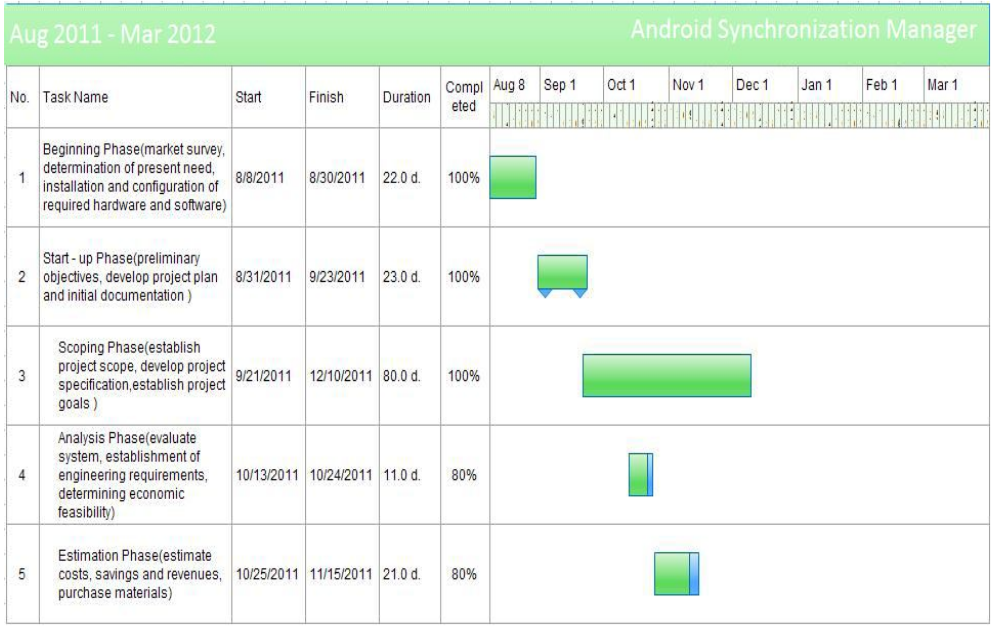
\includegraphics[height= 11cm, width=17cm]{project/images/schedule-A}
  \caption{\textbf{Planning and Scheduling - Part A}}
\end{figure}
\vspace{1cm}
\begin{figure}[H]
  \centering
    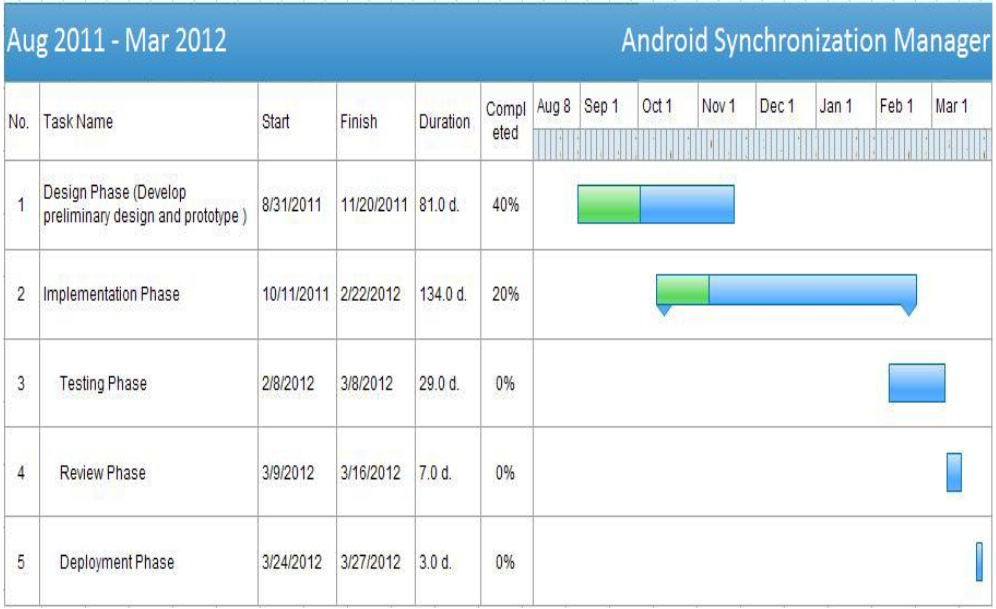
\includegraphics[height= 11cm, width=17cm]{project/images/schedule-B}
  \caption{\textbf{Planning and Scheduling - Part B}}
\end{figure}
\newpage
%\textbf{GitHub}\\
\section{Source Code Management}
\hspace*{0.82cm}For source code management/version control system, we are using GIT. The source code repository are located at GitHub. URL of 
our project for watching or forking is \url{https://github.com/ReverseBitCoders/AndroSync}\\[0.5cm]
\hspace*{0.82cm}GitHub is a web-based hosting service for software development projects that use the Git revision control system. GitHub offers 
both commercial plans and free accounts for open source projects.\\[2cm]

\begin{figure}[H]
  \centering
    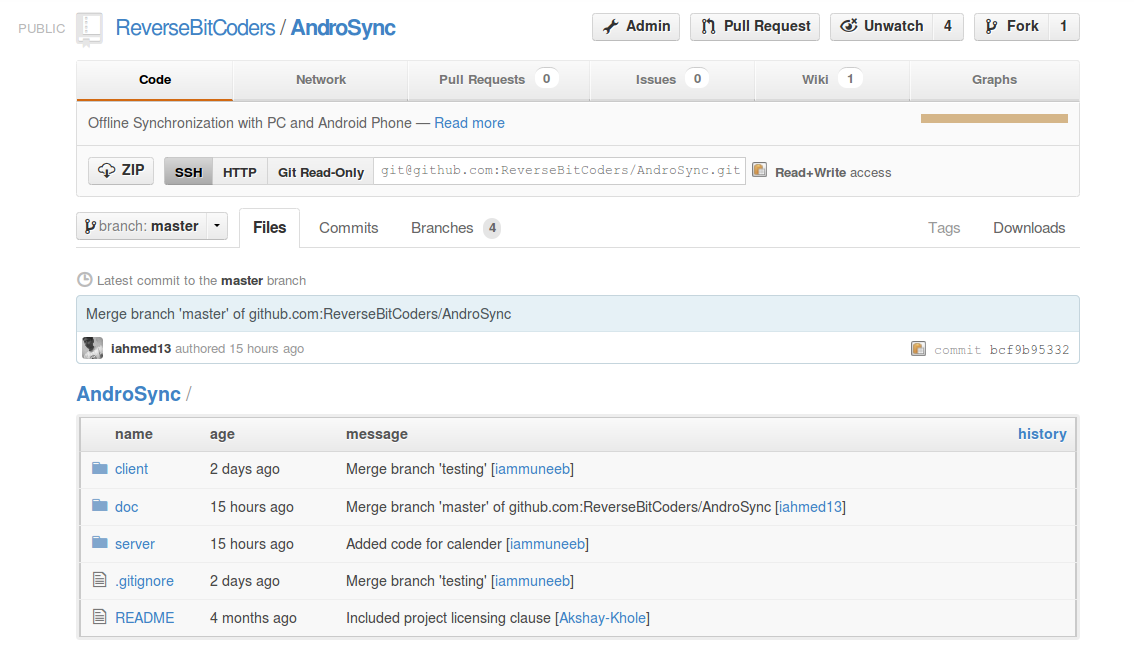
\includegraphics[height= 11cm, width=17cm]{project/images/GitHub/github}
  \caption{\textbf{AndroSync Repository at GitHub}}
\end{figure}

\newpage
\textbf{Progress Graphs generated by GitHub:}\\
\begin{figure}[H]
  \centering
    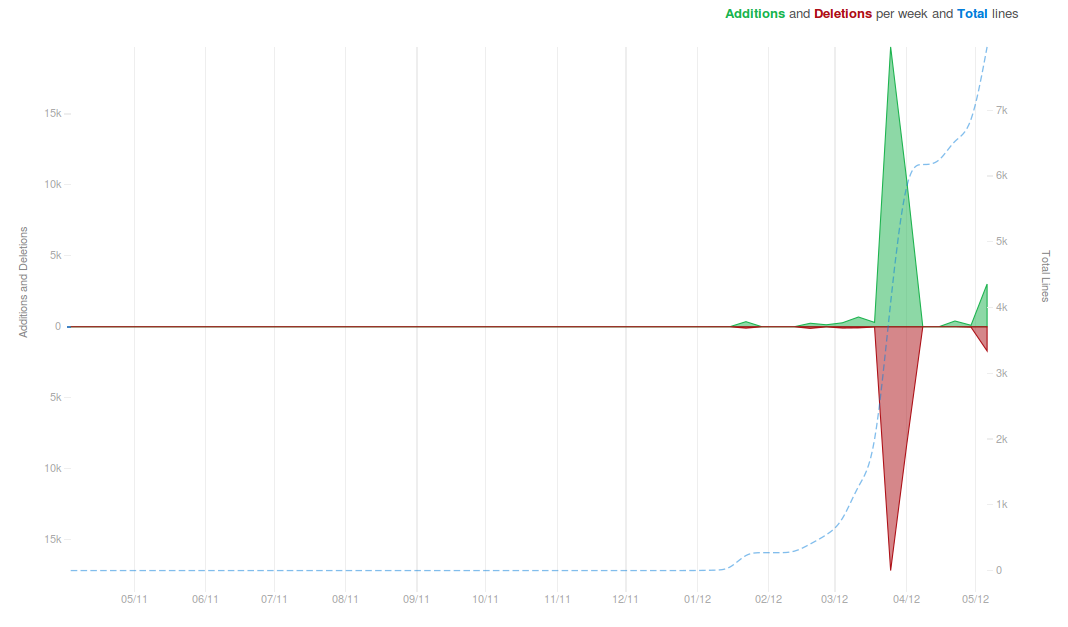
\includegraphics[height= 11cm, width=17cm]{project/images/GitHub/code-freq}
  \caption{\textbf{Code Frequncy}}
\end{figure}
%\vspace{1cm}
\begin{figure}[H]
  \centering
    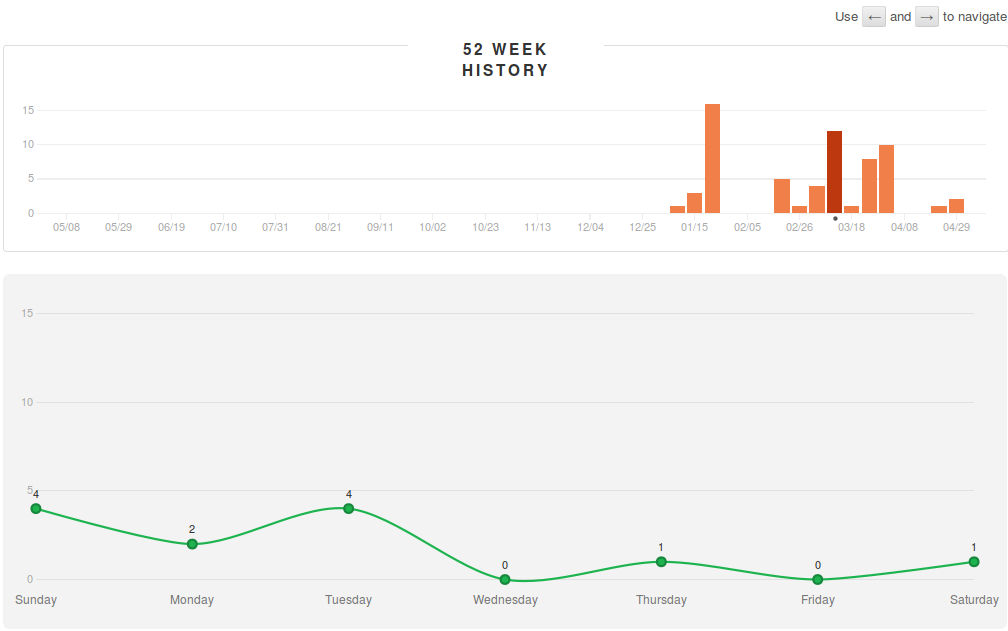
\includegraphics[height= 11cm, width=17cm]{project/images/GitHub/commits}
  \caption{\textbf{Commits}}
\end{figure}
\newpage
\begin{figure}[H]
  \centering
    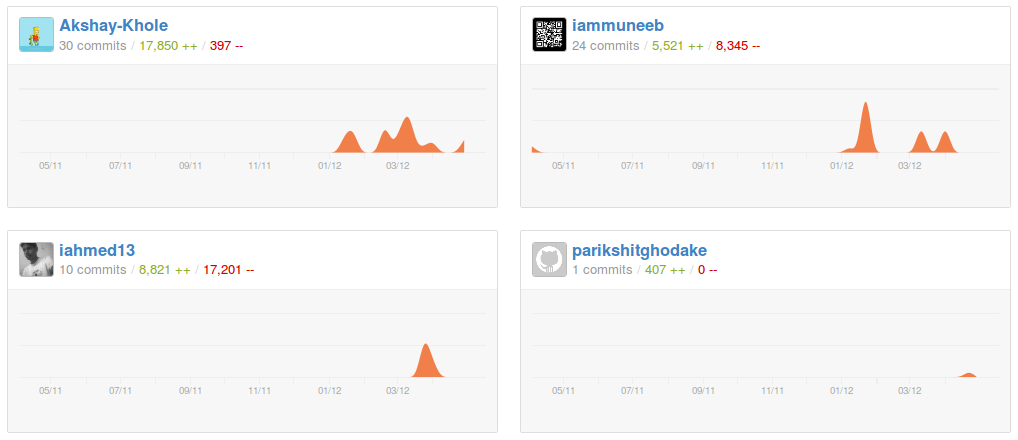
\includegraphics[height= 11cm, width=17cm]{project/images/GitHub/contributors}
  \caption{\textbf{Contributors}}
\end{figure}
\vspace{1cm}
\begin{figure}[H]
  \centering
    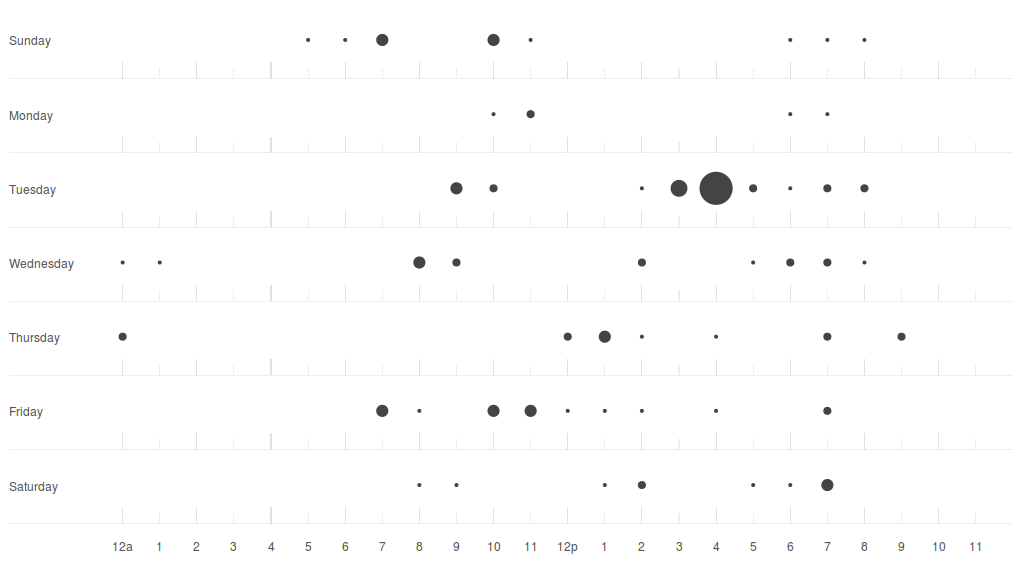
\includegraphics[height= 11cm, width=17cm]{project/images/GitHub/punchcard}
  \caption{\textbf{Punchcard}}
\end{figure}
\newpage
\begin{figure}[H]
  \centering
    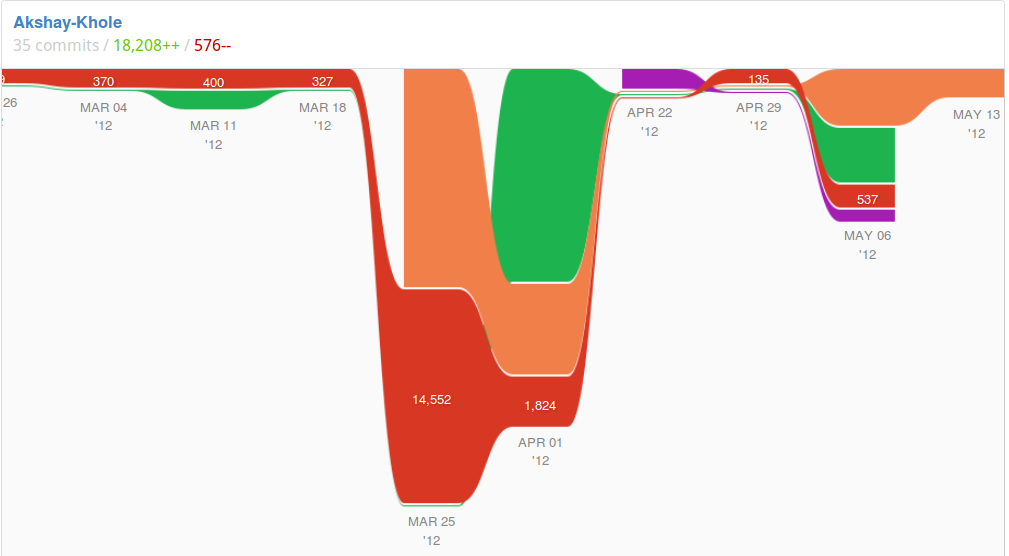
\includegraphics[height= 11cm, width=17cm]{project/images/GitHub/impact-aki}
  \caption{\textbf{Impact - Part A}}
\end{figure}
\vspace{1cm}
\begin{figure}[H]
  \centering
    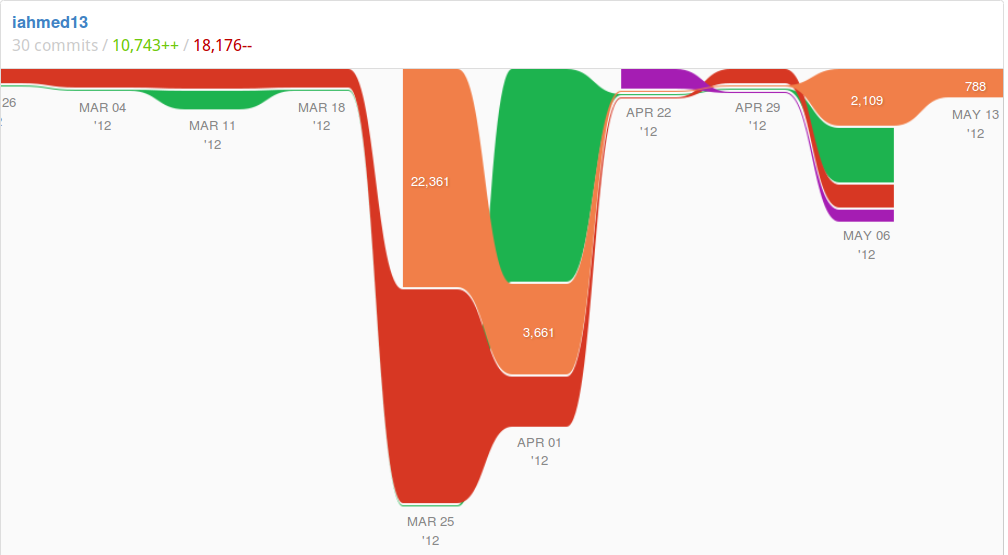
\includegraphics[height= 11cm, width=17cm]{project/images/GitHub/impact-imran}
  \caption{\textbf{Impact - Part B}}
\end{figure}
\newpage
\begin{figure}[H]
  \centering
    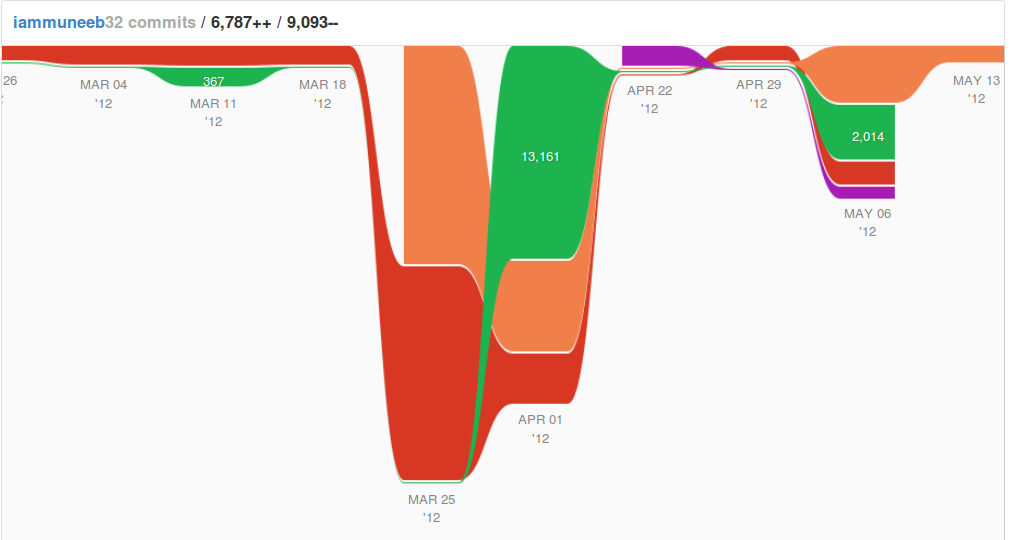
\includegraphics[height= 11cm, width=17cm]{project/images/GitHub/impact-muneeb}
  \caption{\textbf{Impact - Part C}}
\end{figure}
\vspace{1cm}
\begin{figure}[H]
  \centering
    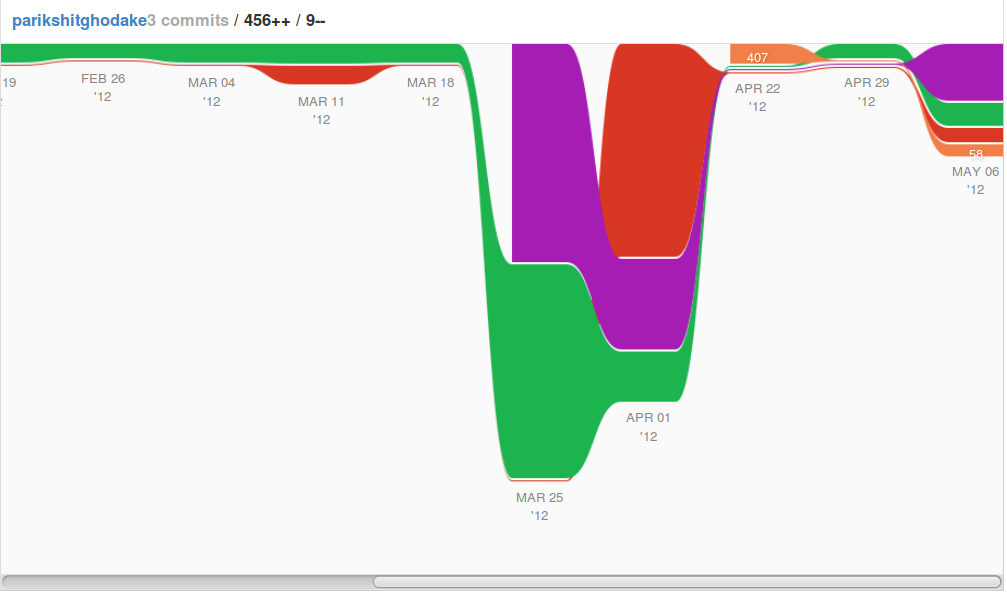
\includegraphics[height= 11cm, width=17cm]{project/images/GitHub/impact-parikshit}
  \caption{\textbf{Impact - Part D}}
\end{figure}